\chapter{酸和碱：Ka 与 pKa}\label{ch:g12:ka-and-pka}

许多蚂蚁用甲酸自卫，甲酸沾在皮肤上时
会灼伤皮肤。甲酸是一种小的
\omterm{def:g11:functional-groups:carboxylic-acid}{羧酸}。同浓度的盐酸会
灼伤得更厉害。两者都是酸，溶液的 \omterm{def:g9:acids-bases-ph:ph}{pH} 都低于 7，但
它们的酸性方式并不相同。要完整描述一种酸，需要两个量：
其一是它的多少，即浓度；其二是它
给出氢\omterm{def:g9:ions:ion}{离子}的难易程度，即\omterm{def:g12:ka-and-pka:ka}{酸度常数}。

\begin{recall}
酸性、碱性和\omterm{def:g9:acids-bases-ph:acidic}{中性溶液}；\omterm{def:g9:acids-bases-ph:ph}{pH} 标度从 0 到 14，
氢\omterm{def:g9:ions:ion}{离子}越多，\omterm{def:g9:acids-bases-ph:ph}{pH} 越低（见\cref{ch:g9:acids-bases-ph}）。
\omterm{def:g12:equilibrium:quotient}{反应商} $Q$ 与\omterm{def:g12:equilibrium:constant}{平衡常数} $K$
（见\cref{ch:g12:equilibrium}）。\omterm{def:g12:curly-arrows:curly-arrow}{弯箭头}表示一对\omterm{def:g9:inside-the-atom:nucleus}{电子}的
移动（见\cref{ch:g12:curly-arrows}）。
\end{recall}

\begin{omfigure}
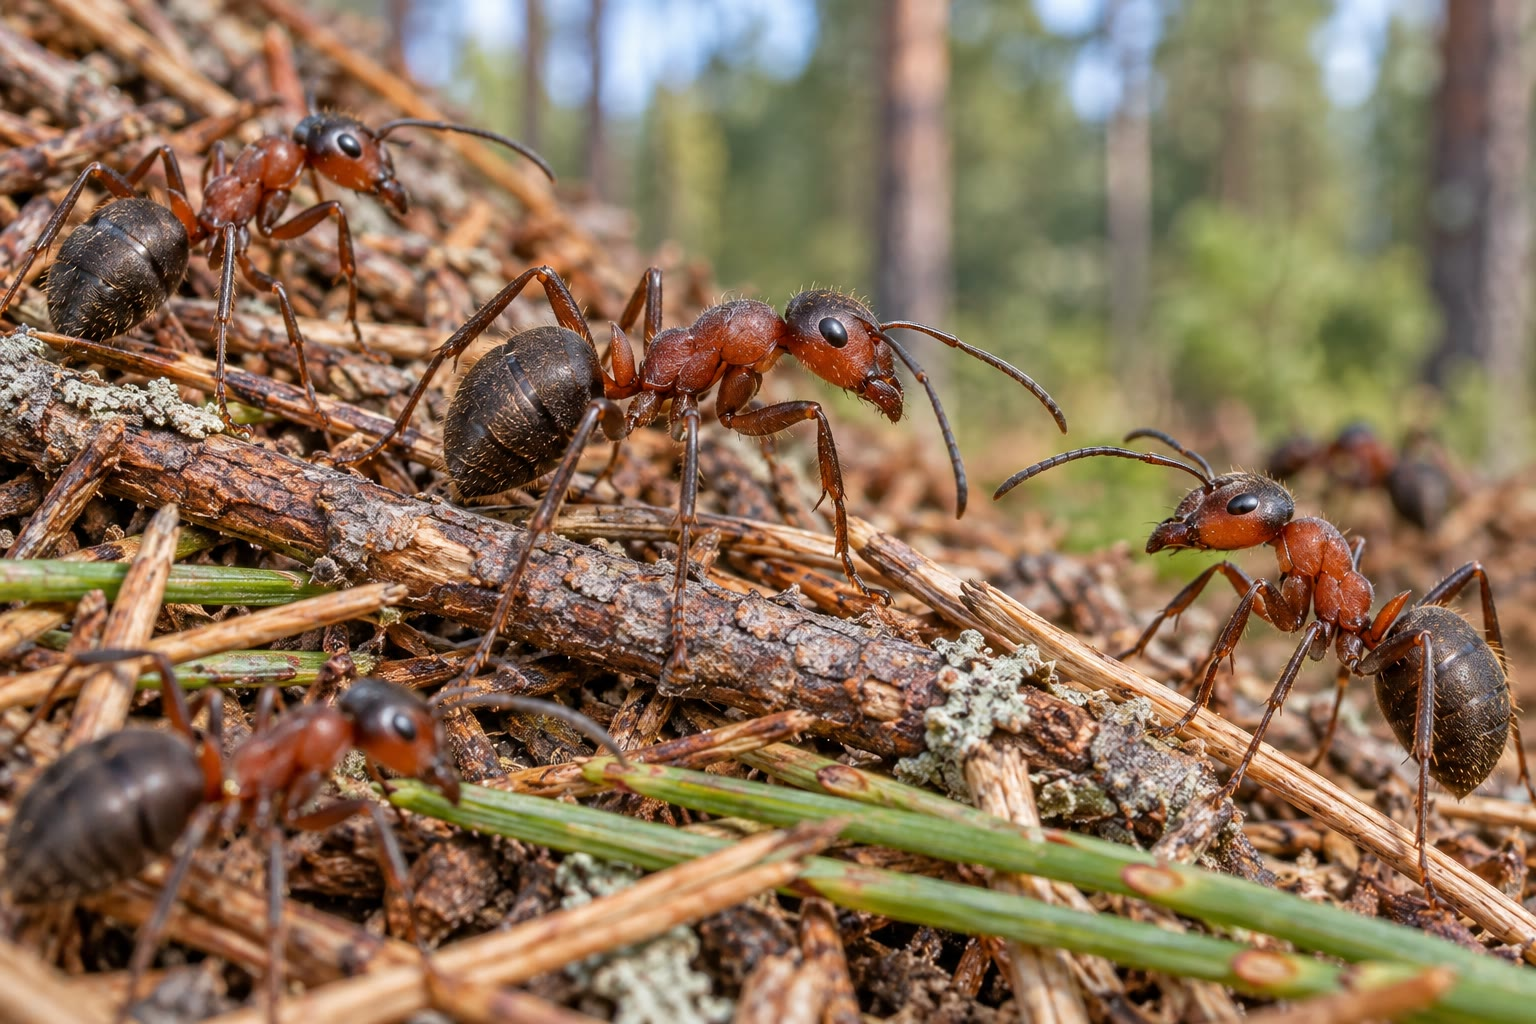
\includegraphics[width=0.45\linewidth]{images/book1/ai/g12-red-ants.jpg}

{\small 林蚁：与许多蚂蚁一样，它们用甲酸自卫。}
\end{omfigure}

\section{布朗斯特酸和碱}

\begin{definition}[布朗斯特酸和碱，酸碱共轭对]\label{def:g12:ka-and-pka:bronsted}
能给出一个氢\omterm{def:g9:ions:ion}{离子} \ce{H+} 的物种称为\emph{布朗斯特酸}\index{布朗斯特酸}；
能接受一个氢\omterm{def:g9:ions:ion}{离子}的物种则称为\emph{布朗斯特碱}\index{布朗斯特碱}。
酸 HA 与由它失去一个氢\omterm{def:g9:ions:ion}{离子}而生成的碱 \ce{A-}，
相差 \ce{H+}，组成一对\emph{酸碱共轭对}\index{酸碱共轭对}，
记作 \ce{HA}/\ce{A-}：$\ce{HA} \rightleftharpoons \ce{A-} + \ce{H+}$。
\end{definition}

\begin{definition}[水合氢离子，两性物质]\label{def:g12:ka-and-pka:oxonium}
在水中，氢\omterm{def:g9:ions:ion}{离子}从不单独存在：它会被一个水\omterm{def:g7:atoms-and-molecules:molecule}{分子}
结合，生成\emph{水合氢离子}\index{水合氢离子} \ce{H3O+}。
既是某一共轭对中的酸、又是另一共轭对中的碱的物种，
称为\emph{两性物质}\index{两性物质}；水即是其中一种，
在共轭对 \ce{H2O}/\ce{OH-} 中为酸，在 \ce{H3O+}/\ce{H2O} 中为碱。
\end{definition}

\begin{example}[水中的酸]\label{ex:g12:ka-and-pka:acid-water}
乙酸\omterm{def:g2:mixing-and-dissolving:dissolve}{溶解}时，水\omterm{def:g7:atoms-and-molecules:molecule}{分子}的一对\omterm{def:g10:lewis-and-shape:lone-pair}{孤电子对}夺取了
乙酸中 \ce{O-H} 的氢，而该 \ce{O-H} 的\omterm{def:g9:inside-the-atom:nucleus}{电子}对留在乙酸\omterm{def:g7:atoms-and-molecules:molecule}{分子}的氧\omterm{def:g7:atoms-and-molecules:atom}{原子}上：
\[
  \ce{CH3COOH + H2O <=> CH3COO- + H3O+} .
\]
两个共轭对交换一个氢\omterm{def:g9:ions:ion}{离子}：\ce{CH3COOH}/\ce{CH3COO-} 给出它，
\ce{H3O+}/\ce{H2O} 接受它。从此以后，前面各章中的氢\omterm{def:g9:ions:ion}{离子}
在以水为\omterm{def:g6:solutions-and-solubility:solute}{溶剂}时，均写作 \ce{H3O+}。
\end{example}

\begin{omfigure}
\setchemfig{atom sep=2em}
\chemfig{H_3C-C(=[2]O)-O-[@{oh}]@{h}H}\qquad
\chemfig{@{ow}\charge{90=\:,270=\:}{O}(-[:150]H)-[:210]H}
\qquad$\longrightarrow$\qquad
\chemfig{H_3C-C(=[2]O)-\charge{90=\:,0=\:,270=\:}{O}^{-}}\quad$+$\quad\ce{H3O+}
\chemmove{
  \draw[->, thick, omProp, shorten <=4pt, shorten >=3pt]
    ($(ow)+(0,0.25)$) .. controls +(110:9mm) and +(60:9mm) .. (h);
  \draw[->, thick, omDef, shorten <=2pt, shorten >=4pt]
    (oh) .. controls +(-90:7mm) and +(-60:6mm) .. ($(oh)+(-0.3,-0.2)$);}

{\small 氢\omterm{def:g9:ions:ion}{离子}由酸转移至水\omterm{def:g7:atoms-and-molecules:molecule}{分子}：水\omterm{def:g7:atoms-and-molecules:molecule}{分子}的一对\omterm{def:g10:lewis-and-shape:lone-pair}{孤电子对}
形成新的 \ce{O-H} 键（橙色），原来的 \ce{O-H} \omterm{def:g9:inside-the-atom:nucleus}{电子}对
留在乙酸根\omterm{def:g9:ions:ion}{离子}的氧\omterm{def:g7:atoms-and-molecules:atom}{原子}上（蓝色）。}
\end{omfigure}

\begin{history}[从阿伦尼乌斯到布朗斯特，1887--1923]
1887 年，斯万特·阿伦尼乌斯提出：酸在水中给出氢\omterm{def:g9:ions:ion}{离子}，
碱则给出氢氧根\omterm{def:g9:ions:ion}{离子}。1923 年，约翰内斯·布朗斯特与
托马斯·劳里各自独立地拓展了这一观点：酸是任何给出氢\omterm{def:g9:ions:ion}{离子}的物种，
碱是任何接受氢\omterm{def:g9:ions:ion}{离子}的物种，无论是否在水中。
氨\omterm{def:g7:atoms-and-molecules:molecule}{分子}中不含氢氧根，却同样成为
一种普通的碱。
\end{history}

\begin{omfigure}
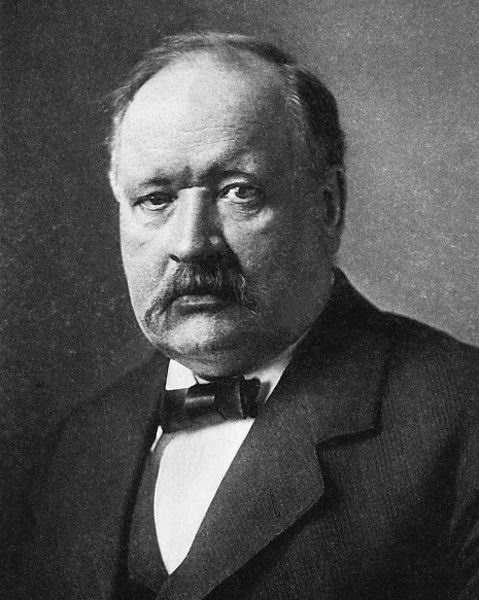
\includegraphics[width=0.22\linewidth]{images/book1/arrhenius.jpg}

{\small 斯万特·阿伦尼乌斯（1859--1927）。}
\end{omfigure}

\section{pH 的定量描述}

\begin{definition}[pH 的精确定义]\label{def:g12:ka-and-pka:ph-log}
在稀\omterm{def:g6:solutions-and-solubility:solute}{水溶液}中，\omterm{def:g9:acids-bases-ph:ph}{pH} 由下式定义：
\[
  \mathrm{pH} = -\log\frac{[\ce{H3O+}]}{c^\circ},
  \qquad\text{即}\qquad
  [\ce{H3O+}] = c^\circ \times 10^{-\mathrm{pH}} ,
\]
其中 $\log$ 为常用对数。
\end{definition}

\begin{proposition}[十倍稀释，相差一个单位]\label{prop:g12:ka-and-pka:dilution}
若 $[\ce{H3O+}]$ 除以 10，则 \omterm{def:g9:acids-bases-ph:ph}{pH} 增加 1；若
乘以 10，则 \omterm{def:g9:acids-bases-ph:ph}{pH} 减少 1。
\end{proposition}

\begin{proof}
$-\log\big([\ce{H3O+}]/10c^\circ\big) = -\log\big([\ce{H3O+}]/c^\circ\big)
+ \log 10 = \mathrm{pH} + 1$.
\end{proof}

\begin{definition}[强酸、弱酸与强碱、弱碱]\label{def:g12:ka-and-pka:strong-acid}
与水\omterm{def:g10:reaction-progress-table:limiting}{完全反应}、溶液中不再存在原来酸\omterm{def:g7:atoms-and-molecules:molecule}{分子}的酸，称为
\emph{强酸}\index{强酸}。与水只部分反应、其反应可达平衡的酸，称为
\emph{弱酸}\index{弱酸}。同样，与水\omterm{def:g10:reaction-progress-table:limiting}{完全反应}的碱称为\emph{强碱}\index{强碱}，
与水只部分反应的碱称为
\emph{弱碱}\index{弱碱}。
\end{definition}

\begin{proposition}[强酸的 pH]\label{prop:g12:ka-and-pka:strong}
浓度为 $c$（不太稀）的\omterm{def:g12:ka-and-pka:strong-acid}{强酸}溶液，
$[\ce{H3O+}] = c$，$\mathrm{pH} = -\log(c/c^\circ)$。
\end{proposition}

\begin{proof}
反应 \ce{HA + H2O -> A- + H3O+} 进行完全：每个酸\omterm{def:g7:atoms-and-molecules:molecule}{分子}
生成一个\omterm{def:g12:ka-and-pka:oxonium}{水合氢离子}。水自身电离产生的\omterm{def:g9:ions:ion}{离子}可以忽略，
只要 $c$ 远大于 \qty{e-7}{mol/L}。
\end{proof}

\begin{example}[盐酸]\label{ex:g12:ka-and-pka:hcl}
盐酸浓度为 \qty{0.010}{mol/L}：$[\ce{H3O+}] = \qty{0.010}{mol/L}$
且 $\mathrm{pH} = -\log 0.010 = 2.0$。\omterm{def:g10:concentration-and-dilution:dilution}{稀释}十倍后，\omterm{def:g9:acids-bases-ph:ph}{pH} 为 3.0。
\end{example}

\section{水与离子积}


\begin{definition}[水的离子积]\label{def:g12:ka-and-pka:ionic-product}
水自身发生的反应极其微弱：\ce{2H2O <=> H3O+ + OH-}。
该反应的\omterm{def:g12:equilibrium:constant}{平衡常数}称为\emph{水的
离子积}\index{水的离子积}：
\[
  K_e = \frac{[\ce{H3O+}]\,[\ce{OH-}]}{(c^\circ)^2},
  \qquad pK_e = -\log K_e .
\]
\end{definition}

\begin{proposition}[中性水与强碱]\label{prop:g12:ka-and-pka:ke}
% ledger: ke:25C
在 \qty{25}{\celsius} 时，$K_e = \num{1.0e-14}$，$pK_e = 14.0$。纯
水中 $[\ce{H3O+}] = [\ce{OH-}] = \qty{1.0e-7}{mol/L}$，\omterm{def:g9:acids-bases-ph:ph}{pH} 为 7.0。
\omterm{def:g12:ka-and-pka:strong-acid}{强碱}浓度为 $c$ 时，$[\ce{OH-}] = c$，于是
$[\ce{H3O+}] = K_e (c^\circ)^2 / c$，$\mathrm{pH} = 14.0 + \log(c/c^\circ)$。
\end{proposition}

\begin{proof}
纯水中两种\omterm{def:g9:ions:ion}{离子}成对产生，因此二者相等，它们的
乘积为 $\num{1.0e-14}$，各为 \qty{1.0e-7}{mol/L}。对于碱，
溶液中 $K_e$ 仍然成立：
$-\log([\ce{H3O+}]/c^\circ) = -\log K_e + \log(c/c^\circ)$.
\end{proof}

\begin{example}[氢氧化钠]\label{ex:g12:ka-and-pka:naoh}
氢氧化钠浓度为 \qty{0.010}{mol/L}：$[\ce{OH-}] = 0.010$，于是
$[\ce{H3O+}] = \num{1.0e-14}/0.010 = \qty{1.0e-12}{mol/L}$，\omterm{def:g9:acids-bases-ph:ph}{pH} 为 12.0。
\end{example}

\section{酸度常数}

\begin{definition}[酸度常数，$pK_a$]\label{def:g12:ka-and-pka:ka}
\emph{酸度常数}\index{酸度常数} $K_a$ 为\omterm{def:g12:ka-and-pka:bronsted}{酸碱共轭对}
\ce{HA}/\ce{A-} 的酸与水反应的
\omterm{def:g12:equilibrium:constant}{平衡常数}，即 \ce{HA + H2O <=> A- + H3O+}：
\[
  K_a = \frac{[\ce{A-}]\,[\ce{H3O+}]}{[\ce{HA}]\,c^\circ} .
\]
该共轭对的\emph{pKa}\index{pKa} 为
$pK_a = -\log K_a$。
\end{definition}

\begin{proposition}[$pK_a$ 越小，酸越强]\label{prop:g12:ka-and-pka:compare}
在浓度相同的两种\omterm{def:g12:ka-and-pka:strong-acid}{弱酸}中，
$K_a$ 较大（即 $pK_a$ 较小）的那种与水反应更多，
溶液的 \omterm{def:g9:acids-bases-ph:ph}{pH} 更低；其共轭碱则更弱。
\end{proposition}

\begin{proof}
$K_a$ 越大，平衡时 \ce{A-} 与 \ce{H3O+} 越多，
对于同一 \ce{HA}。易放出氢\omterm{def:g9:ions:ion}{离子}的酸，其共轭碱 \ce{A-}
则较难再结合氢\omterm{def:g9:ions:ion}{离子}。
\end{proof}

\begin{omfigure}
\begin{tikzpicture}[font=\small, y=0.55cm]
  % ledger: pka:methanoic, pka:ethanoic, pka:benzoic, pka:ascorbic1, ka:HF, ka:H2CO3, ka:HCO3, kb:NH3, ke:25C
  \draw[->, thick] (0,0) -- (0,14.8) node[above] {$pK_a$};
  \foreach \k in {0,2,4,6,8,10,12,14} \draw (-0.1,\k) -- (0.1,\k) node[right, font=\scriptsize] {\k};
  \node[font=\footnotesize\bfseries, anchor=south] at (-3.0,14.3) {酸};
  \node[font=\footnotesize\bfseries, anchor=south] at (3.0,14.3) {碱};
  \foreach \p/\yl/\acid/\base in {3.19/2.9/{\ce{HF}}/{\ce{F-}},
      3.74/3.6/{\ce{HCOOH}}/{\ce{HCOO-}}, 4.04/4.3/{抗坏血酸}/{抗坏血酸根},
      4.20/5.0/{\ce{C6H5COOH}}/{\ce{C6H5COO-}}, 4.76/5.7/{\ce{CH3COOH}}/{\ce{CH3COO-}},
      6.37/6.9/{\ce{CO2,H2O}}/{\ce{HCO3-}}, 9.26/9.26/{\ce{NH4+}}/{\ce{NH3}},
      10.33/10.4/{\ce{HCO3-}}/{\ce{CO3^{2-}}}} {
    \draw[omDef] (-0.25,\p) -- (0.25,\p);
    \draw[black!40] (-0.25,\p) -- (-1.1,\yl);
    \draw[black!40] (0.25,\p) -- (1.1,\yl);
    \node[anchor=east, font=\scriptsize] at (-1.15,\yl) {\acid};
    \node[anchor=west, font=\scriptsize] at (1.15,\yl) {\base};
  }
  \draw[->, omThm, thick] (-4.6,13) -- (-4.6,1);
  \node[omThm, rotate=90, font=\footnotesize] at (-4.95,7) {较强的酸};
  \draw[->, omMeth, thick] (4.6,1) -- (4.6,13);
  \node[omMeth, rotate=90, font=\footnotesize] at (4.95,7) {较强的碱};
\end{tikzpicture}

{\small 若干共轭对按其 $pK_a$ 排列（\qty{25}{\celsius}），酸在左，
碱在右。位置越低，其酸越强；越高，
其碱越强。}
\end{omfigure}


\begin{method}[弱酸的 pH]\label{met:g12:ka-and-pka:weak}
设\omterm{def:g12:ka-and-pka:strong-acid}{弱酸}浓度为 $c$、\omterm{def:g12:ka-and-pka:ka}{酸度常数}为 $K_a$：
\begin{enumerate}
  \item 按每升计，写出 \ce{HA + H2O <=> A- + H3O+} 的\omterm{def:g10:reaction-progress-table:extent}{进度表}，
        其中 $x = [\ce{H3O+}]$，$[\ce{HA}] = c - x$，$[\ce{A-}] = x$
        （忽略水自身电离产生的\omterm{def:g9:ions:ion}{离子}）。
  \item 解方程 $\dfrac{x^2}{(c - x)\,c^\circ} = K_a$，即二次方程
        $x^2 + K_a c^\circ x - K_a c^\circ c = 0$，
        并取其正根。
  \item $\mathrm{pH} = -\log(x/c^\circ)$；检验 $x$ 远大于
        \qty{e-7}{mol/L}。
\end{enumerate}
\end{method}

\begin{example}[\texorpdfstring{\qty{0.010}{mol/L}}{0.010 mol/L} 浓度下的乙酸]\label{ex:g12:ka-and-pka:acetic}
% ledger: pka:ethanoic
$pK_a = 4.76$，故 $K_a = 10^{-4.76} = \num{1.74e-5}$。于是
$x^2 + \num{1.74e-5}\,x - \num{1.74e-7} = 0$ 解得
$x = \qty{4.1e-4}{mol/L}$，\omterm{def:g9:acids-bases-ph:ph}{pH} 为 3.39。仅有 $\num{4.1e-4}/0.010 =
\qty{4.1}{\percent}$ 的酸已与水反应；同浓度的盐酸
\omterm{def:g9:acids-bases-ph:ph}{pH} 为 2.0，已\omterm{def:g10:reaction-progress-table:limiting}{完全反应}。
\end{example}

\begin{omfigure}
\begin{tikzpicture}[font=\small]
  \fill[omThm!45] (0,1.3) rectangle (8,2.0);
  \node[anchor=east] at (-0.1,1.65) {盐酸 \ce{HCl}，\qty{0.010}{mol/L}};
  \node[white, font=\small\bfseries] at (4,1.65) {\ce{H3O+} + \ce{Cl-}：\qty{100}{\percent}};
  \fill[omDef!35] (0,0) rectangle (7.67,0.7);
  \fill[omThm!45] (7.67,0) rectangle (8,0.7);
  \node[anchor=east] at (-0.1,0.35) {乙酸 \ce{CH3COOH}，\qty{0.010}{mol/L}};
  \node at (3.8,0.35) {\ce{CH3COOH} 保持原样：\qty{95.9}{\percent}};
  \draw[<-, omThm] (7.85,0.75) -- (8.4,1.1) node[right, font=\footnotesize] {\qty{4.1}{\percent} 电离};
\end{tikzpicture}

{\small 同浓度的\omterm{def:g12:ka-and-pka:strong-acid}{强酸}与\omterm{def:g12:ka-and-pka:strong-acid}{弱酸}各会怎样：
\omterm{def:g12:ka-and-pka:strong-acid}{强酸}全部转化为\omterm{def:g9:ions:ion}{离子}，\omterm{def:g12:ka-and-pka:strong-acid}{弱酸}则几乎不电离。
由此得到两者的 \omterm{def:g9:acids-bases-ph:ph}{pH} 差，即 2.0 与 3.4。}
\end{omfigure}

\begin{safety}{\ghs[0.75cm]{GHS02}\ghs[0.75cm]{GHS05}\ghs[0.75cm]{GHS06}\ghs[0.75cm]{GHS07}}
% ledger: ghs:formic-acid
浓甲酸易燃，会严重灼伤皮肤
和眼睛，其蒸气有毒。仅由教师
在通风橱内操作；练习中的稀溶液仍需
佩戴护目镜。
\end{safety}

\section{练习}

\begin{exercise}[$\star$]\label{exo:g12:ka-and-pka:1}
写出下列物质的共轭碱：\ce{HCOOH}、\ce{NH4+}、\ce{H2O}、\ce{HCO3-}；
并写出下列物质的共轭酸：\ce{NH3}、\ce{OH-}、\ce{H2O}、\ce{HCO3-}。
哪些粒子是\omterm{def:g12:ka-and-pka:oxonium}{两性物质}？
\end{exercise}

\begin{exercise}[$\star$]\label{exo:g12:ka-and-pka:2}
求下列浓度盐酸的 \omterm{def:g9:acids-bases-ph:ph}{pH}：\qty{0.10}{mol/L}、
\qty{0.0010}{mol/L} 和 \qty{5.0e-3}{mol/L}。
\end{exercise}

\begin{exercise}[$\star$]\label{exo:g12:ka-and-pka:3}
某溶液的 \omterm{def:g9:acids-bases-ph:ph}{pH} 为 4.5，求 $[\ce{H3O+}]$。另一溶液的 \omterm{def:g9:acids-bases-ph:ph}{pH} 为 11.2：
求 \qty{25}{\celsius} 时的 $[\ce{H3O+}]$ 和 $[\ce{OH-}]$。
\end{exercise}

\begin{exercise}[$\star$]\label{exo:g12:ka-and-pka:4}
写出甲酸与水反应的方程式及 $K_a$ 的表达式，
并对铵根\omterm{def:g9:ions:ion}{离子}作同样处理。
\end{exercise}

\begin{exercise}[$\star$]\label{exo:g12:ka-and-pka:5}
哪一种酸较强：甲酸（$pK_a = 3.74$）还是乙酸
（$pK_a = 4.76$）？哪一种碱较强：\ce{HCOO-} 还是
\ce{CH3COO-}？
\end{exercise}

\begin{exercise}[$\star\star$]\label{exo:g12:ka-and-pka:6}
某\omterm{def:g12:ka-and-pka:strong-acid}{弱酸} HA 的溶液浓度为 \qty{0.050}{mol/L}，\omterm{def:g9:acids-bases-ph:ph}{pH} 为 3.0。求
$[\ce{A-}]$、$[\ce{HA}]$，再求 $K_a$ 与 $pK_a$。
\end{exercise}

\begin{exercise}[$\star\star$]\label{exo:g12:ka-and-pka:7}
求 \qty{0.020}{mol/L} 苯甲酸（$pK_a = 4.20$）的 \omterm{def:g9:acids-bases-ph:ph}{pH}。
\end{exercise}

\begin{exercise}[$\star\star$]\label{exo:g12:ka-and-pka:8}
求 \qty{2.0e-3}{mol/L} 氢氧化钠溶液的 \omterm{def:g9:acids-bases-ph:ph}{pH}。
\end{exercise}

\begin{exercise}[$\star\star$]\label{exo:g12:ka-and-pka:9}
利用 $pK_a$ 标度，将图中所示共轭对的酸
按由强到弱排列。像 \ce{HCl} 这样的\omterm{def:g12:ka-and-pka:strong-acid}{强酸}
应位于何处？
\end{exercise}

\begin{exercise}[$\star\star$]\label{exo:g12:ka-and-pka:10}
溶于水的二氧化碳使水略显酸性（共轭对
\ce{CO2,H2O}/\ce{HCO3-}，$pK_a = 6.37$）。一份与\omterm{def:g4:air-a-mixture-of-gases:air}{空气}接触的雨水样品
测得 \omterm{def:g9:acids-bases-ph:ph}{pH} 为 5.6。求 $[\ce{H3O+}]$，并与纯水比较。
\end{exercise}

\begin{exercise}[$\star\star$]\label{exo:g12:ka-and-pka:11}
证明对共轭对 \ce{NH4+}/\ce{NH3}，有 $pK_a = pK_e - pK_b$，其中
$K_b = \num{1.8e-5}$ 是 \ce{NH3 + H2O <=> NH4+ + OH-} 的\omterm{def:g12:equilibrium:constant}{平衡常数}。
求 $pK_a$。
\end{exercise}

\begin{exercise}[$\star\star\star$]\label{exo:g12:ka-and-pka:12}
乙酸的浓度为 \qty{0.010}{mol/L}，\omterm{def:g9:acids-bases-ph:ph}{pH} 为 3.39。求
\omterm{def:g10:concentration-and-dilution:dilution}{稀释}十倍后的 \omterm{def:g9:acids-bases-ph:ph}{pH}。它是否如\omterm{def:g12:ka-and-pka:strong-acid}{强酸}那样上升一个单位？
请说明理由。
\end{exercise}

\begin{exercise}[$\star\star\star$]\label{exo:g12:ka-and-pka:13}
碳酸氢根\omterm{def:g9:ions:ion}{离子}是\omterm{def:g12:ka-and-pka:oxonium}{两性物质}。写出它与水的两个反应，
并利用 $pK_a$ 标度写出其\omterm{def:g12:equilibrium:constant}{平衡常数}。哪一个更大？
由此可推测碳酸氢钠溶液的
\omterm{def:g9:acids-bases-ph:ph}{pH} 应如何？
\end{exercise}

\begin{exercise}[$\star\star\star$]\label{exo:g12:ka-and-pka:14}
将 \qty{1.0e-3}{mol/L} 的盐酸\omterm{def:g10:concentration-and-dilution:dilution}{稀释}一千倍，
再\omterm{def:g10:concentration-and-dilution:dilution}{稀释}一千倍。若草率套用规则，先得 \omterm{def:g9:acids-bases-ph:ph}{pH} 6，再得
\omterm{def:g9:acids-bases-ph:ph}{pH} 9。为何\omterm{def:g10:concentration-and-dilution:dilution}{稀释}后的酸不可能达到 \omterm{def:g9:acids-bases-ph:ph}{pH} 9？极稀溶液的
\omterm{def:g9:acids-bases-ph:ph}{pH} 趋近于何值？
\end{exercise}

\begin{exercise}[$\star\star\star$]\label{exo:g12:ka-and-pka:15}
抗坏血酸（维生素 C，$pK_a = 4.04$，$M = \qty{176.0}{g/mol}$）：将
一片 \qty{500}{mg} 的药片溶于 \qty{200}{mL} 水中。计算
其 \omterm{def:g9:acids-bases-ph:ph}{pH}（只考虑第一步电离）。
\end{exercise}

\section{问题：蚂蚁的毒液}


\begin{problem}[{周末问题——蚂蚁毒液中的甲酸
在 0.010 mol/L 时 pH 为多少，小苏打如何缓解其灼痛？}]
\label{pb:g12:ka-and-pka:1}
% ledger: src:formic-ants, pka:methanoic, ka:H2CO3, ke:25C, aw:C, aw:H, aw:O
甲酸 \ce{HCOOH} 存在于蚂蚁的毒液中。其 $pK_a$ 在
\qty{25}{\celsius} 时为 3.74。研究浓度为 \qty{0.010}{mol/L} 的溶液，并
将其与盐酸作比较。

\medskip
\noindent\textbf{第一部分——酸。}
\begin{enumerate}
  \item 画出甲酸的\omterm{def:g10:lewis-and-shape:lewis-structure}{路易斯结构}，并圈出
        它给出的氢。
  \item 写出其共轭对及其与水的反应。
  \item 写出 $K_a$ 并计算其值。
  \item 将该共轭对置于 $pK_a$ 标度上：甲酸
        比乙酸更强还是更弱？
  \item 计算 \qty{1.0}{L} 该溶液中甲酸的
        质量。
\end{enumerate}

\medskip
\noindent\textbf{第二部分——\omterm{def:g9:acids-bases-ph:ph}{pH}。}
\begin{enumerate}[resume]
  \item 以每升计填写\omterm{def:g10:reaction-progress-table:extent}{进度表}，其中 $x = [\ce{H3O+}]$。
  \item 写出方程 $Q_{eq} = K_a$。
  \item 解该方程。
  \item 计算 \omterm{def:g9:acids-bases-ph:ph}{pH}。
  \item 有多大比例的酸与水发生了反应？
  \item 检验来自水的\omterm{def:g9:ions:ion}{离子}可以忽略不计。
\end{enumerate}

\medskip
\noindent\textbf{第三部分——比较。}
\begin{enumerate}[resume]
  \item \qty{0.010}{mol/L} 盐酸的 \omterm{def:g9:acids-bases-ph:ph}{pH} 是多少？
  \item 它所含的\omterm{def:g12:ka-and-pka:oxonium}{水合氢离子}是
        甲酸溶液的多少倍？
  \item 用“强”和“弱”两词解释其差异。
\end{enumerate}

\medskip
\noindent\textbf{第四部分——小苏打。}
\begin{enumerate}[resume]
  \item 小苏打是碳酸氢钠。写出
        甲酸与碳酸氢根\omterm{def:g9:ions:ion}{离子}之间的反应（生成甲酸根和
        \ce{CO2,H2O}）。
  \item 证明其常数为 $K = K_a(\ce{HCOOH}) / K_a(\ce{CO2,H2O})$，
        并计算其值。
  \item 该反应是否有利？可观察到什么气体？
  \item 为何比氢氧根弱得多的碱（例如碳酸氢根）
        更适合用于皮肤？
  \item 给出最终答案：\qty{0.010}{mol/L} 的
        甲酸溶液的 \omterm{def:g9:acids-bases-ph:ph}{pH} 是多少？
\end{enumerate}
\end{problem}
